\chapter{ПРОТОКОЛ СИМЕТРИЧНОЇ КРИПТОСИСТЕМИ}\label{ch:-3:---}

Спираючись на теоретичні основи скінченних кілець, відображень та систем лінійних рівнянь, розглянуті у Розділі~2, у цьому розділі подано конкретний протокол обміну інформацією для симетричної криптосистеми.
Спочатку окреслюється необхідний етап налаштування, включаючи початкову домовленість щодо секретних параметрів і генерацію потрібних алгебраїчних компонентів.
Далі наведено покроковий опис дій, які виконують сторони, що обмінюються повідомленнями (традиційно — Аліса і Боб), під час шифрування та дешифрування.
Ілюстративний приклад демонструє роботу протоколу на конкретних параметрах.
Після цього розглядається криптоаналіз протоколу, аналізуються можливі вектори атак і оцінюється стійкість на основі аргументів, наведених у попередніх розділах.
Нарешті, обговорюються практичні аспекти реалізації, обчислювальна ефективність і можливі варіації чи вдосконалення основного протоколу.


\section{Огляд протоколу та етап налаштування}
\label{sec:protocol_overview}
Основна мета протоколу — забезпечити захищений обмін повідомленнями між двома сторонами, Алісою і Бобом, які мають спільний набір початкових секретних параметрів.
Стійкість ґрунтується на симетричній природі ключового матеріалу, отриманого з цих параметрів, і обчислювальній складності для зловмисника відновити відкритий текст із перехопленого шифротексту без знання цих секретів.
Загальна архітектура, що включає декілька кілець ($Z_m, G_m, G_k$) та відображень ($\varphi, \psi, \lambda, \psi_1, \lambda_1$), як показано на рис.~\ref{fig:schema} і розглянуто у~\ref{subsec:system_diagram}, забезпечує основу для роботи протоколу, дозволяючи виконувати обчислення в ефективних доменах, а зовнішньо представляти дані в обфускованому вигляді.

\subsection{Початкова домовленість щодо ключа та генерація параметрів}
\label{subsec:protocol_setup}

Перш ніж розпочати захищене спілкування, Аліса і Боб повинні встановити спільний секретний ключ.
Це досягається на етапі налаштування, що вимагає попереднього захищеного каналу (наприклад, фізичний обмін, захищений протокол узгодження ключа~\cite{24}).
Під час цього етапу вони погоджують такі початкові секретні параметри:
\begin{itemize}
    \item Параметри $(a, c, l, k)$, необхідні для алгоритму GEN-G (див.~\ref{subsec:gen_g_algorithm}).
    Тут $k$ — порядок більшого кільця $G_k$, $m = k/l$ — порядок робочого кільця $G_m$, а $a, c$ — коефіцієнти, для яких $\gcd(a, k) = 1$.
    \item Конкретні, погоджені правила перетворення, які застосовуються на відповідному кроці алгоритму GEN-G.
    Це критично для отримання ідентичних структур обома сторонами.
\end{itemize}
Використовуючи ці спільні секрети, Аліса і Боб незалежно виконують алгоритм GEN-G:
\begin{itemize}
    \item Вони запускають GEN-G$(a, c, l, m)$ (або адаптують запуск для $k$) з погодженими правилами перетворення для генерації визначального рядка для $G_m$.
    Це неявно визначає кільце $G_m$ та ключовий ізоморфізм $\varphi: Z_m \to G_m$.
    \item Вони запускають GEN-G$(a, c, l, k)$ з погодженими правилами для генерації визначального рядка для більшого кільця $G_k$.
\end{itemize}
Оскільки використовуються однакові вхідні дані та детермінований алгоритм, включаючи ідентичні секретні правила перетворення, обидві сторони гарантовано отримують однакові кільця $G_m, G_k$ та один і той самий ізоморфізм $\varphi$.

Окрім кілець та $\varphi$, для повної функціональності протоколу необхідно також визначити інші відображення, показані на рис.~\ref{fig:schema}: сюр'єкції $\psi, \lambda: G_k \to G_m$ та відповідні бієкції фактор-множин $\psi_1: G_k/\psi \to G_m$, $\lambda_1: G_k/\lambda \to G_m$.
Ці відображення також мають бути погоджені між Алісою і Бобом на етапі налаштування або детерміновано виведені зі спільних секретів $(a,c,l,k)$ за попередньо узгодженим правилом.
Крім того, секретні параметри для афінного перетворення, яке використовує Аліса (матриці $B_i$ та вектори $a_j$), також мають бути встановлені як частина спільного ключового матеріалу.
Повний спільний секретний ключ таким чином складається з $(a,c,l,k)$, правил GEN-G, визначень $\psi, \lambda, \psi_1, \lambda_1$ та послідовності $(B_i, a_j)$. Огляд етапу налаштування та генерації спільного ключа представлено на рис.~\ref{fig:setup_overview}.

\begin{figure}[ht]
    \centering
    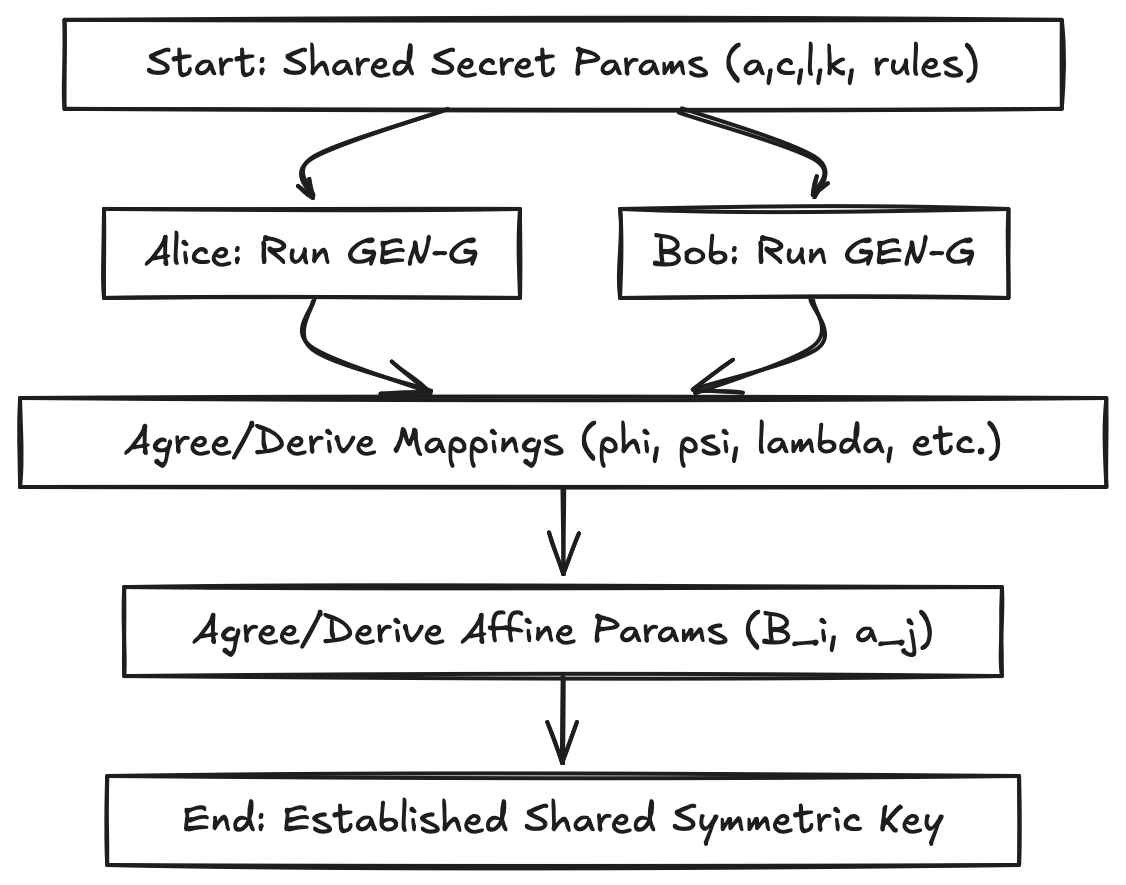
\includegraphics[width=0.3\textheight,keepaspectratio]{pictures/Setup Phase Overview Diagram}
    \caption{Огляд етапу налаштування та генерації спільного ключа.}
    \label{fig:setup_overview}
\end{figure}

\subsection{Вибір шляху комунікації}
\label{subsec:communication_paths}

Архітектура системи, зображена на рис.~\ref{fig:schema}, дозволяє гнучко використовувати відображення для зовнішнього представлення.
Можливі три основні шляхи створення шифрограми залежно від того, які фактор-множини використовуються для представлення публічних систем і фінального шифротексту:
\begin{enumerate}
    \item \textbf{Шлях 1:} $G_k/\psi \to G_m \to Z_m \to G_m$.
    Публічні системи $l(x), L(x)$ представлені у $G_k/\psi$.
    Боб переводить їх через $\psi_1^{-1}$ та $\varphi^{-1}$ у $Z_m$ для обчислень.
    Отримані компоненти шифротексту $d, d_1$ (у $Z_m$) відображаються через $\varphi$ у $G_m$ для передачі (або далі).
    \item \textbf{Шлях 2:} $G_k/\lambda \to G_m \to Z_m \to G_k/\psi$.
    Публічні системи $l(x), L(x)$ представлені у $G_k/\lambda$.
    Боб переводить їх через $\lambda_1^{-1}$ та $\varphi^{-1}$ у $Z_m$ для обчислень.
    Отримані компоненти шифротексту $d, d_1$ (у $Z_m$) відображаються через $\varphi$ у $G_m$, далі через $\psi_1$ у $G_k/\psi$ для передачі як представників із $G_k$.
    \item \textbf{Шлях 3:} $G_k/\psi \to G_m \to Z_m \to G_k/\lambda$.
    Публічні системи $l(x), L(x)$ представлені у $G_k/\psi$.
    Боб переводить їх через $\psi_1^{-1}$ та $\varphi^{-1}$ у $Z_m$ для обчислень.
    Отримані компоненти шифротексту $d, d_1$ (у $Z_m$) відображаються через $\varphi$ у $G_m$, далі через $\lambda_1$ у $G_k/\lambda$ для передачі як представників із $G_k$.
\end{enumerate}
Вибір шляху впливає на те, які саме відображення ($\lambda_1^{-1}$ чи $\psi_1^{-1}$ для вхідних даних, $\psi_1$ чи $\lambda_1$ для вихідних) використовуються на інтерфейсах.
Детальний опис протоколу далі відповідає Шляху~2, згідно з основним викладом у попередніх розділах.


\section{Деталізовані кроки протоколу}
\label{sec:protocol_steps}
Після етапу налаштування протокол передбачає три основні інтерактивні кроки.
Нижче описано дії Аліси (яка готує системи та дешифрує) і Боба (який шифрує повідомлення).

\subsection{Крок 1: Аліса — побудова систем і публікація}
\label{subsec:protocol_step1_alice}
Аліса готує основу для обміну, налаштовуючи та публікуючи необхідні системи, використовуючи спільний секретний ключовий матеріал.
\begin{enumerate}
    \item[\textbf{1a.}] \textbf{Побудова базової системи $l(x)$:} Аліса визначає початкову лінійну систему $l(x) = Ax$ над кільцем $G_m$.
    Тут $A$ — матриця розмірності $p \times q$, де $p$ — розмір блоку відкритого тексту, а $q \geq p$ — кількість змінних.
    Аліса повинна забезпечити, щоб $A$ задовольняла умови розв'язності, описані у~\ref{subsec:sle_solvability_rings}: рядки $A$ мають бути лінійно незалежними за модулем $m$, а в $A$ має бути обернена підматриця $A_1$ розмірності $p \times p$.
    Перевірка незалежності здійснюється розв'язанням $A^T y \equiv 0 \pmod{m}$ (єдиний розв'язок — нульовий).
    Далі визначаються $p$ лінійно незалежних стовпців, що утворюють підматрицю $A_1$ з $\gcd(\det(A_1), m) = 1$.
    \item[\textbf{1b.}] \textbf{Застосування секретних афінних перетворень:} Аліса застосовує послідовність з $r \geq 1$ секретних афінних перетворень до $l(x)$, отримуючи перетворену систему $L(x)$.
    Для цього вона використовує секретну послідовність обернених матриць $B_1, \ldots, B_r$ розмірності $p \times p$ та секретні вектори $a_1, \ldots, a_{r+1}$ розмірності $p \times 1$ (усі над $G_m$):
    \[
        L(x) = B_r(B_{r-1}(\ldots B_2(B_1(l(x)+a_1)+a_2)\ldots + a_{r-1})+a_r)+a_{r+1}
    \]
    Обчислення виконуються у $G_m$, зазвичай через ізоморфізм $\varphi$ у $Z_m$.
    В результаті $L(x)$ має афінний вигляд $L(x) = Bx + a$ для деяких $B, a$.
    \item[\textbf{1c.}] \textbf{Обфускація систем для публікації:} Аліса готує системи до публікації.
    Відповідно до обраного шляху (наприклад, Шлях~2), вона використовує відображення $\lambda_1: G_k/\lambda \to G_m$.
    Для кожного коефіцієнта у матрицях $A, B$ та кожної компоненти вектора $a$ (усі в $G_m$) вона знаходить відповідний клас у $G_k/\lambda$ через $\lambda_1^{-1}$ і вибирає представника з цього класу у $G_k$.
    Системи, утворені цими представниками, позначаються $\bar{l}(x) = \bar{A}x$ та $\bar{L}(x) = \bar{B}x + \bar{b}$.
    \item[\textbf{1d.}] \textbf{Публікація систем:} Аліса робить обфусковані системи $\bar{l}(x)$ і $\bar{L}(x)$ загальнодоступними, наприклад, надсилає їх Бобу відкритим каналом або розміщує на вебсайті.
\end{enumerate}

\subsection{Крок 2: Боб — шифрування та передача}
\label{subsec:protocol_step2_bob}
Боб використовує публічні системи Аліси та спільні секрети для шифрування свого повідомлення.
\begin{enumerate}
    \item[\textbf{2a.}] \textbf{Відновлення систем у $Z_m$:} Боб отримує публічні системи $\bar{l}(x) = \bar{A}x$ і $\bar{L}(x) = \bar{B}x + \bar{b}$ з коефіцієнтами у $G_k$.
    Використовуючи спільні секретні відображення для обраного шляху, він спочатку застосовує сюр'єкцію $\lambda: G_k \to G_m$ (відповідає $\lambda_1^{-1}$), а потім ізоморфізм $\varphi^{-1}: G_m \to Z_m$, отримуючи системи у $Z_m$: $\hat{l}(x) = \hat{A}x$, $\hat{L}(x) = \hat{B}x + \hat{a}$.
    \item[\textbf{2b.}] \textbf{Шифрування блоку повідомлення:} Боб перетворює своє повідомлення у послідовність числових значень (наприклад, за табл.~\ref{tab:alphabet}) і ділить на блоки $v$ довжини $p$.
    Для кожного блоку $v$ він виконує:
    \begin{itemize}
        \item Розв'язує базову систему $\hat{l}(x) = v$ ($\hat{A}x \equiv v \pmod{m}$), знаходячи розв'язок $\bar{x} \in Z_m^q$.
        \item Вибирає новий випадковий вектор $\bar{a} \in Z_m^q$, незалежно для кожного блоку.
        \item Обчислює першу компоненту шифротексту $d = \hat{l}(\bar{a}) = \hat{A}\bar{a} \pmod{m}$.
        \item Обчислює другу компоненту шифротексту $d_1 = \hat{L}(\bar{x} + \bar{a}) = \hat{B}(\bar{x} + \bar{a}) + \hat{a} \pmod{m}$.
    \end{itemize}
    \item[\textbf{2c.}] \textbf{Обфускація та передача шифротексту:} Боб зберігає блок відкритого тексту $v$ у таємниці.
    Він обфускує обчислені компоненти шифротексту $d, d_1$ (вектори у $Z_m$) для передачі.
    Відповідно до обраного шляху, спочатку відображає їх у $G_m$ через $\varphi$, далі через бієкцію $\psi_1: G_k/\psi \to G_m$ знаходить відповідні класи у $G_k/\psi$, вибирає представників з цих класів у $G_k$ для формування переданих векторів $(\bar{d}, \bar{d}_1)$.
    Цю пару Боб надсилає Алісі відкритим каналом.
    Кроки 2b і 2c повторюються для кожного блоку повідомлення, причому для кожного блоку використовується новий випадковий вектор $\bar{a}$.
\end{enumerate}

\subsection{Крок 3: Аліса — дешифрування}
\label{subsec:protocol_step3_alice}
Аліса отримує послідовність пар шифротексту від Боба і використовує свій секретний ключовий матеріал для дешифрування кожної з них.
\begin{enumerate}
    \item[\textbf{3a.}] \textbf{Відновлення основних компонент шифротексту:} Для кожної отриманої пари $(\bar{d}, \bar{d}_1)$ (елементи $G_k$) Аліса використовує зворотні відображення для обраного шляху.
    Вона застосовує сюр'єкцію $\psi: G_k \to G_m$ (концептуально $\psi_1^{-1}$), а потім ізоморфізм $\varphi^{-1}: G_m \to Z_m$, отримуючи вектори $d, d_1$ у $Z_m$.
    \item[\textbf{3b.}] \textbf{Обчислення обернених перетворень:} Аліса знає секретні матриці $B_1, \ldots, B_r$, які використовувалися в афінному перетворенні.
    Вона обчислює їх обернені $B_1^{-1}, \ldots, B_r^{-1}$ у $G_m$ або, частіше, обернені $\hat{B}_i^{-1}$ їхніх еквівалентів у $Z_m$ ($\hat{B}_i = \varphi^{-1}(B_i)$) за допомогою ефективних алгоритмів (див.~\ref{subsec:matrix_ops_zm}).
    \item[\textbf{3c.}] \textbf{Зворотне перетворення та відновлення відкритого тексту:} Аліса виконує дешифрувальні обчислення, описані у~\ref{subsec:decryption_mechanism}.
    Використовуючи обернені матриці $\hat{B}_i^{-1}$ та відомі секретні вектори $\hat{a}_j = \varphi^{-1}(a_j)$, вона зворотно відтворює афінне перетворення, застосоване до $d_1$, отримуючи проміжне значення $v_{intermediate} = \hat{l}(\bar{x} + \bar{a}) + \hat{a}_1$.
    Далі вона обчислює остаточний результат:
    \[
        v = v_{intermediate} - (d + \hat{a}_1)
    \]
    Як показано раніше, це дає $v = \hat{l}(\bar{x})$, тобто початковий блок відкритого тексту.
    Аліса повторює цей процес для всіх отриманих пар шифротексту, відновлюючи повне повідомлення.
\end{enumerate}
Коректність цього процесу дешифрування випливає з властивостей афінних перетворень та лінійності $l(x)$, як було доведено у~\ref{sec:core_mechanism}.


\section{Ілюстративний приклад}
\label{sec:protocol_example}
Для наочності роботи протоколу розглянемо детальний числовий приклад, що демонструє всі основні етапи налаштування, шифрування та дешифрування.

\textbf{Етап налаштування:}
\begin{itemize}
    \item \textbf{Початкові параметри:} Аліса і Боб погоджують параметри для GEN-G: $a=7$, $c=5$, $l=2$, $k=50$.
    Модуль робочого кільця $m = k/l = 25$.
    Також погоджуються секретні правила перетворення для кроку~2 GEN-G.
    \item \textbf{Кодування символів:} Для перетворення тексту у числові блоки використовується кодування символів алфавіту згідно з табл.~\ref{tab:alphabet}.
    \item \textbf{Генерація $G_{25}$ та ізоморфізму $\varphi$:} GEN-G з параметрами $(7, 5, 1, 25)$ (або адаптація запуску для $k=50$) і спільними правилами дає визначальний рядок для $G_{25}$:
    \begin{equation*}
      \begin{multlined}
        b_{G_{25}} = (1, 6, 8, 10, 2, 4, 3, 5, 7, 9, 11, 13, 15, 17, 19, \\
                   21, 12, 14, 16, 18, 20, 24, 22, 23, 0)
      \end{multlined}
    \end{equation*}
    Це визначає ізоморфізм $\varphi: Z_{25} \to G_{25}$, наприклад, $\varphi(0)=0$, $\varphi(1)=1$, $\varphi(2)=6$, \ldots, $\varphi(24)=23$.
    \item \textbf{Генерація $G_{50}$:} GEN-G з $(7, 5, 2, 50)$ і спільними правилами дає визначальний рядок для $G_{50}$.
    \item \textbf{Визначення відображень $\psi, \psi_1$:} Погоджується сюр'єкція $\psi: G_{50} \to G_{25}$ та відповідна бієкція $\psi_1: G_{50}/\psi \to G_{25}$.
    Для кожного $j \in \{0, \ldots, 24\}$ (елемент у $G_{25}$ через $\varphi$) вказується два елементи з $G_{50}$ (представники класу у $G_{50}/\psi$).
    \item \textbf{Кодування символів:} Погоджується відповідність символів алфавіту елементам $Z_{25}$ (наприклад, $a=0$, $b=1$, \ldots, $z=24$).
\end{itemize}

\begin{table}[ht]
  \centering
  \small 
  \setlength{\tabcolsep}{3pt}
  \begin{tabular}{|*{25}{c|}}
  \hline 
  0 & 1 & 2 & 3 & 4 & 5 & 6 & 7 & 8 & 9 & 10 & 11 & 12 & 13 & 14  &
  15 & 16 & 17 & 18 & 19 & 20 & 21 & 22 & 23 &  24\\
  \hline
  a & b & c & d & e & f & g & h & i/j & k & l & m & n & o & p & q &
  r & s & t & u & v & w & x & y & z\\
  \hline
  \end{tabular}
  \caption{Цифрові відповідники символів алфавіту}
  \label{tab:alphabet}
\end{table}

Аліса також секретно обирає параметри афінного перетворення: $r=1$, матриця $B_1 = \begin{pmatrix}
                                                                                       6 & 1 \\ 23 & 23
\end{pmatrix}$ у $G_{25}$, вектор $a_1 = (1, 2)^t$ у $G_{25}$.
Вона обчислює еквіваленти у $Z_{25}$: $\bar{B}_1 = \begin{pmatrix}
                                                                                                                      2 & 1 \\ -1 & -1
\end{pmatrix}$, $\hat{a}_1 = (1, 2)^t$, і перевіряє, що $\bar{B}_1$ обернена ($\det(\bar{B}_1) = -1 \equiv 24$, взаємно просте з 25).

\textbf{Виконання протоколу:}

\textbf{Крок 1 (Аліса):}
\begin{itemize}
    \item[\textbf{1a.}] Аліса визначає $l(x) = Ax$ у $G_{25}$. У $Z_{25}$ це $\hat{l}(x) = \hat{A}x$, де
    \[
        \hat{A} = \begin{pmatrix}
                      5 & 6 & 9 & 21 \\ 0 & 1 & 11 & 14
        \end{pmatrix}
    \]
    Вона перевіряє, що матриця задовольняє умови розв'язності (наприклад, стовпці 2 і 3 утворюють підматрицю з визначником $6 \cdot 11 - 9 \cdot 1 = 66 - 9 = 57 \equiv 7 \pmod{25}$, $\gcd(7,25)=1$).
    \item[\textbf{1b.}] Аліса обчислює перетворену систему $L(x) = B_1(l(x) + a_1)$ у $G_{25}$. У $Z_{25}$ це $\hat{L}(x) = \bar{B}_1(\hat{l}(x) + \hat{a}_1)$:
    \[
        \hat{L}(x) = \begin{pmatrix}
                         10x_1 + 13x_2 + 4x_3 + 6x_4 + 7 \\ 20x_1 + 18x_2 + 5x_3 + 15x_4 + 19
        \end{pmatrix}
    \]
    \item[\textbf{1c.}] Аліса обфускує коефіцієнти $l(x)$ і $L(x)$ через відображення у $G_{50}/\psi$, вибираючи представників з $G_{50}$ для кожного коефіцієнта. Наприклад:
    \begin{gather*}
        \bar{l}(x) = \begin{cases}
                         17x_1 + 34x_2 + 21x_3 + 26x_4 \\ 7x_1 + 14x_2 + 42x_3 + 43x_4
        \end{cases}\\
        \bar{L}(x) = \begin{cases}
                         48x_1 + 41x_2 + 3x_3 + 46x_4 + 19 \\ 15x_1 + 32x_2 + 44x_3 + 36x_4 + 30
        \end{cases}\\
    \end{gather*}
    (Коефіцієнти — елементи $G_{50}$, подані як цілі числа 0–49).
    \item[\textbf{1d.}] Аліса публікує $\bar{l}(x)$ і $\bar{L}(x)$.
\end{itemize}

\textbf{Крок 2 (Боб):}
\begin{itemize}
    \item[\textbf{2a.}] Боб отримує $\bar{l}(x), \bar{L}(x)$ і за допомогою зворотних відображень ($\psi^{-1}$, $\varphi^{-1}$) відновлює системи у $Z_{25}$:
    \begin{gather*}
        \hat{l}(x) = \begin{cases}
                         5x_1 + 6x_2 + 9x_3 + 21x_4 \\ 0x_1 + 1x_2 + 11x_3 + 14x_4
        \end{cases}\\
        \hat{L}(x) = \begin{cases}
                         10x_1 + 13x_2 + 4x_3 + 6x_4 + 7 \\ 20x_1 + 18x_2 + 5x_3 + 15x_4 + 19
        \end{cases}\\
    \end{gather*}
    \item[\textbf{2b.}] Боб шифрує повідомлення "tara tara tarara".
    Блоки відкритого тексту (за табл.~\ref{tab:alphabet}): $v_1=(18,0)$ [ta], $v_2=(16,0)$ [ra], $v_3=(18,0)$ [ta], $v_4=(16,0)$ [ra] тощо.

    \textbf{Шифрування блоку 1 ($v_1=(18,0)$):}
    \begin{itemize}
        \item Розв'язує $\hat{l}(x) = (18, 0)$: $\bar{x} = (0, 14, 1, 0)$.
        \item Вибирає випадковий $\bar{a} = (0, 1, 0, 1)$.
        \item Обчислює $d = \hat{l}(\bar{a}) = (5 \cdot 0 + 6 \cdot 1 + 9 \cdot 0 + 21 \cdot 1, 0 \cdot 0 + 1 \cdot 1 + 11 \cdot 0 + 14 \cdot 1) = (27, 15) \equiv (2, 15) \pmod{25}$.
        \item $\bar{x} + \bar{a} = (0, 15, 1, 1)$.
        \item $d_1 = \hat{L}(0, 15, 1, 1) = (10 \cdot 0 + 13 \cdot 15 + 4 \cdot 1 + 6 \cdot 1 + 7, 20 \cdot 0 + 18 \cdot 15 + 5 \cdot 1 + 15 \cdot 1 + 19) = (212, 309) \equiv (12, 9) \pmod{25}$.
    \end{itemize}
    \item[\textbf{2c.}] Боб обфускує $d=(2,15)$, $d_1=(12,9)$ (з $Z_{25}$) у $G_{25}$ через $\varphi$, далі у $G_{50}/\psi$ через $\psi_1$, вибирає представників $\bar{d}, \bar{d}_1$ з $G_{50}$ і передає їх Алісі.
\end{itemize}

\textbf{Крок 3 (Аліса — дешифрування блоку 1):}
\begin{itemize}
    \item[\textbf{3a.}] Аліса отримує обфусковану пару, застосовує зворотні відображення ($\psi^{-1}$, $\varphi^{-1}$), відновлює $d = (2, 15)$, $d_1 = (12, 9)$ у $Z_{25}$.
    \item[\textbf{3b.}] Обчислює обернену до $\bar{B}_1$ у $Z_{25}$:
    \[
        \bar{B}_1^{-1} = \begin{pmatrix}
                             1 & 1 \\ -1 & -2
        \end{pmatrix} \pmod{25}
    \]
    \item[\textbf{3c.}] Виконує дешифрування з використанням $\hat{a} = (7, 19)^t$:
    \begin{itemize}
        \item $d_1' = d_1 - \hat{a} = (12, 9) - (7, 19) = (5, -10) \equiv (5, 15) \pmod{25}$.
        \item $v_{intermediate} = \bar{B}_1^{-1} d_1' = (1 \cdot 5 + 1 \cdot 15, -1 \cdot 5 - 2 \cdot 15) = (20, -35) \equiv (20, 15) \pmod{25}$.
        \item $v = v_{intermediate} - d = (20, 15) - (2, 15) = (18, 0) \pmod{25}$.
    \end{itemize}
    Аліса відновлює $v_1 = (18, 0)$, що відповідає "ta".
    На рисунку~\ref{fig:data_trace_example} показано приклад трасування перетворень для одного числового значення через різні кільця та відображення.
\end{itemize}

\begin{figure}[ht]
    \centering
    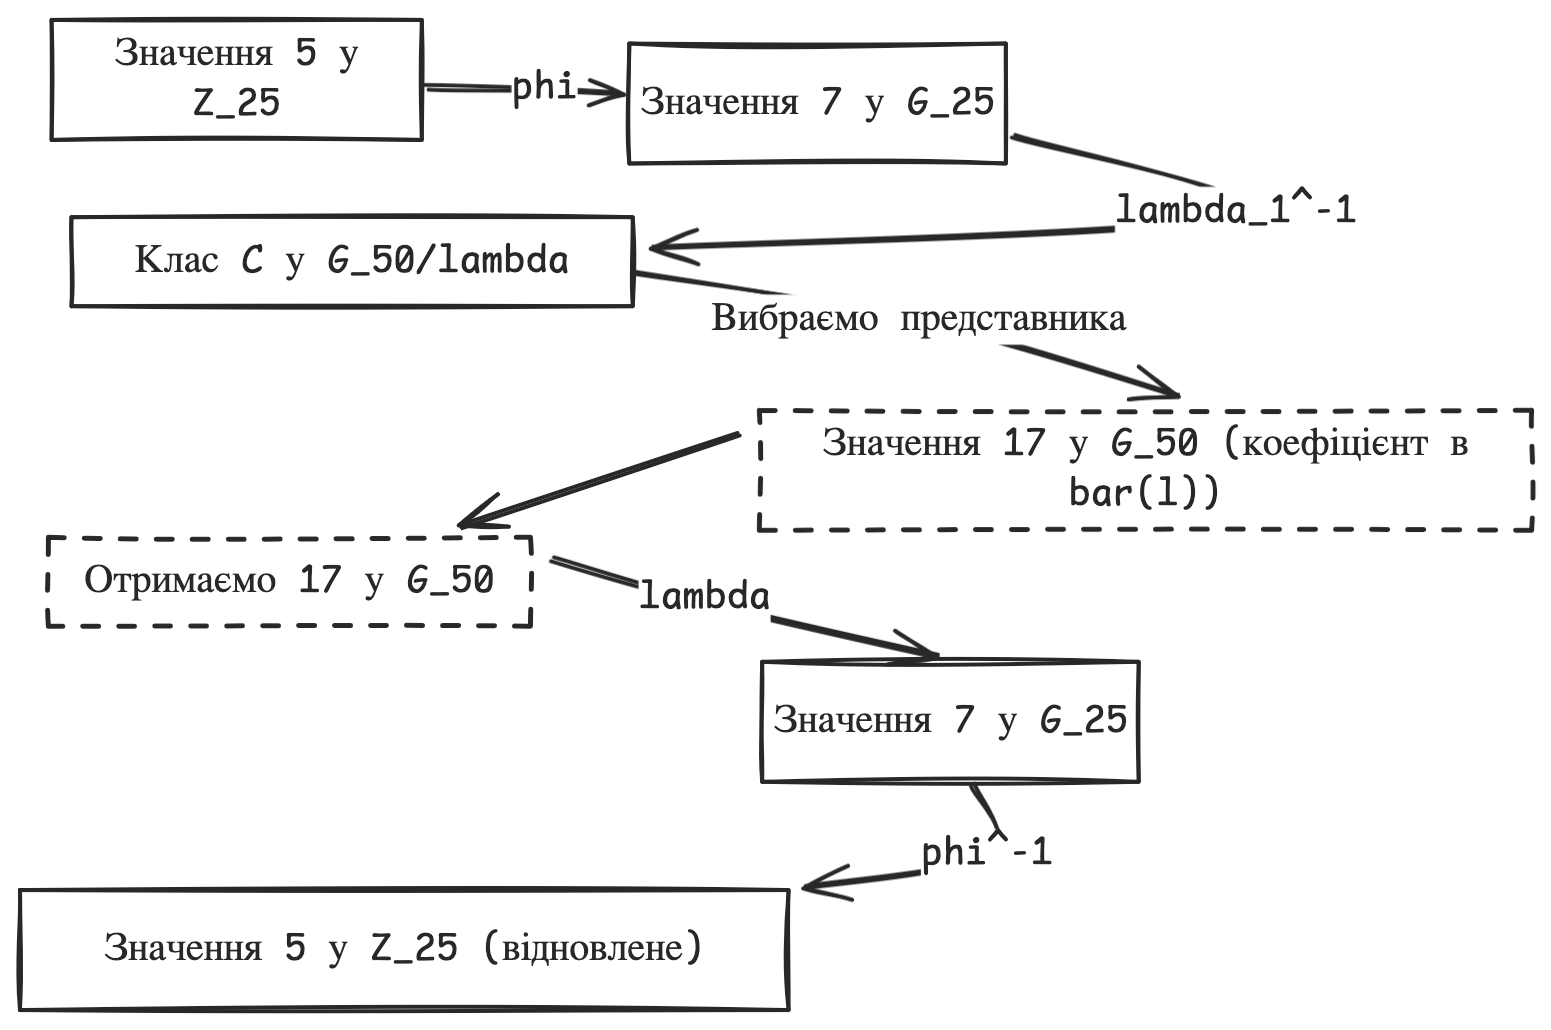
\includegraphics[width=\textwidth]{pictures/Example Data Trace Diagram}
    \caption{Приклад трасування перетворень для одного числового значення.}
    \label{fig:data_trace_example}
\end{figure}

\textbf{Шифрування/дешифрування наступних блоків:}
\begin{itemize}
    \item \textbf{Блок 2 ("ra", $v_2=(16,0)$):}
    \begin{itemize}
        \item $\bar{x}=(0,18,12,0)$, $\bar{a}=(1,0,1,0)$.
        \item $d=(14,11)$, $d_1=(3,3)$.
        \item $\bar{B}_1^{-1}(d_1-\hat{a})^t = (5,11)$, $v = (5,11)-(14,11) = (-9,0) \equiv (16,0)$.
    \end{itemize}
    \item \textbf{Блок 3 ("ta", $v_3=(18,0)$), новий $\bar{a}$:}
    \begin{itemize}
        \item $\bar{x}=(0,14,1,0)$, $\bar{a}=(0,0,1,1)$.
        \item $d=(5,0)$, $d_1=(3,21)$.
        \item $\bar{B}_1^{-1}(d_1-\hat{a})^t = (23,0)$, $v = (23,0)-(5,0) = (18,0)$.
    \end{itemize}
    \item \textbf{Блок 4 ("ra", $v_4=(16,0)$), новий $\bar{a}$:}
    \begin{itemize}
        \item $\bar{x}=(0,18,12,0)$, $\bar{a}=(0,0,0,1)$.
        \item $d=(21,14)$, $d_1=(20,18)$.
        \item $\bar{B}_1^{-1}(d_1-\hat{a})^t = (12,14)$, $v = (12,14)-(21,14) = (-9,0) \equiv (16,0)$.
    \end{itemize}
\end{itemize}
Процедура повторюється для всіх блоків.
Фінальна послідовність пар шифротексту $(d, d_1)$ у $Z_{25}$: $((2,15), (12,9)), ((14,11), (3,3)), ((5,0), (3,21)), ((21,14), (20,18)), \ldots$.
Після дешифрування всіх пар Аліса відновлює числову послідовність відкритого тексту $(18,0), (16,0), (18,0), (16,0), \ldots$ і перетворює її у повідомлення "tara tara tarara".

Цей приклад підкреслює необхідність використання нового випадкового вектора $\bar{a}$ для кожного блоку, навіть для повторюваних блоків відкритого тексту, щоб забезпечити різні шифротексти.
Також продемонстровано, що дешифрування успішно відновлює відкритий текст шляхом зворотного афінного перетворення із застосуванням секретної оберненої матриці $\bar{B}_1^{-1}$ та віднімання випадкової компоненти $d$.


\section{Криптоаналіз протоколу}
\label{sec:protocol_cryptanalysis}
У цьому розділі аналізується стійкість запропонованого протоколу до основних типів криптоаналітичних атак.
Розглядається точка зору зовнішнього атакуючого, який має доступ до публічної інформації (системи, шифротексти) та знає загальний алгоритм, але не володіє секретними параметрами.

\subsection{Інформація, доступна атакуючому}
\label{subsec:attacker_knowledge}
Відповідно до принципу Керкгоффса, атакуючий знає всі алгоритми, але не конкретний секретний ключ.
Згідно з описом протоколу (див.~\ref{sec:protocol_steps}), атакуючому доступна така інформація:
\begin{enumerate}
    \item \textbf{Публічні системи:} Обфусковані системи $\bar{l}(x)$ та $\bar{L}(x)$ з коефіцієнтами у $G_k$ (тобто числа від $0$ до $k-1$). З $\bar{L}(x)$ можна визначити кількість рівнянь $p$ та кількість змінних $q$.
    \item \textbf{Шифротексти:} Послідовність пар $(\bar{d}_i, \bar{d}_{i1})$, де кожна компонента — елемент $G_k$.
    \item \textbf{Порядки кілець:} Можливо, відомі або визначаються порядки $m$ і $k$ кілець $Z_m$ ($G_m$) та $Z_k$ ($G_k$).
    \item \textbf{Структура протоколу:} Відомі ролі $l(x), L(x)$, випадкового вектора $\bar{a}$, відображень тощо.
\end{enumerate}
Недоступною для атакуючого є така інформація:
\begin{enumerate}
    \item Конкретні параметри $(a, c)$ і секретні правила перетворення для GEN-G.
    \item Відповідний ізоморфізм $\varphi: Z_m \to G_m$.
    \item Сюр'єкції $\psi, \lambda: G_k \to G_m$.
    \item Бієкції $\psi_1: G_k/\psi \to G_m$, $\lambda_1: G_k/\lambda \to G_m$.
    \item Секретні матриці $B_i$ і вектори $a_j$ для афінного перетворення.
    \item Випадкові вектори $\bar{a}_i$ для кожного блоку.
    \item Блоки відкритого тексту $v_i$.
\end{enumerate}

\subsection{Можливі вектори атаки}
\label{subsec:attack_vectors}
Розглянемо основні типи атак, які може застосувати атакуючий.

\subsubsection{1. Атака повним перебором} \\
\label{subsubsec:brute_force}

Атака полягає у систематичному переборі всіх можливих комбінацій секретних компонентів ключа для відновлення відкритого тексту.

Загальна кількість комбінацій для лише відображень оцінюється як
\[
(m-2)!\cdot m! \cdot \frac{k!}{m!(l!)^m},
\]
де $(m-2)!$ — кількість можливих ізоморфізмів $\varphi$, $m!$ — кількість бієкцій $\psi_1$ (або $\lambda_1$), а $\frac{k!}{m!(l!)^m}$ — кількість сюр'єкцій $\psi$ (або $\lambda$), де $k=lm$.

Навіть для відносно невеликих параметрів ця кількість є астрономічною.
Наприклад, для $m=25$, $k=50$, $l=2$:
\begin{equation*}
    23! \cdot 25! \cdot \frac{50!}{25! \cdot 2^{25}} = \frac{23! \cdot 50!}{2^{25}} > 2^{94} > 10^{31}\, \text{сек}.
\end{equation*}
Якщо припустити, що одна комбінація перевіряється за $10^{-14}$ секунд, то повний перебір займе понад $10^{31}$ секунд, тобто більше ніж $10^7$ років.

Додавання перебору афінних параметрів ($B_i, a_j$) ще більше збільшує складність.
Таким чином, атака повним перебором є обчислювально нездійсненною навіть для невеликих порядків кілець; збільшення $m$ і $k$ робить її ще менш реальною.

\subsubsection{2. Атаки з відомим відкритим текстом або шифротекстом} \\
\label{subsubsec:known_plaintext}

Розглянемо два сценарії:

\paragraph{2.1. Атака лише за шифротекстом.} \\
Атакуючий має доступ до багатьох пар шифротексту $(\bar{d}_i, \bar{d}_{i1})$ для невідомих відкритих текстів. Відомо, що ці пари пов'язані з внутрішніми значеннями $(d_i, d_{i1})$ через невідомі відображення ($\varphi, \psi_1$ тощо). Однак для відновлення відкритого тексту необхідно знати ці відображення та секретні перетворення ($B_i, a_j$). Простір можливих відображень має розмір, пов'язаний з $(m-2)! \times m! \times \frac{k!}{m!(l!)^m}$, і навіть наявність багатьох шифротекстів не зменшує суттєво складність пошуку потрібних секретних відображень. Шифротексти у $G_k$ не дають прямої інформації про структуру $G_m$ чи $Z_m$ без правильних зворотних відображень.

\paragraph{2.2. Атака з відомим відкритим текстом.} \\
Атакуючий має декілька пар відомих блоків відкритого тексту $v_i$ та відповідних обфускованих шифротекстів $(\bar{d}_i, \bar{d}_{i1})$. Зв'язок між ними задається через невідомі відображення ($\xi, \varphi, \psi_1$), і атакуючий не може легко отримати основні компоненти шифротексту $(d_i, d_{i1})$ у $Z_m$. Навіть якщо це вдасться, рівняння $d_i = \hat{l}(\bar{a}_i)$, $d_{i1} = \hat{L}(\bar{x}_i + \bar{a}_i)$, де $v_i = \hat{l}(\bar{x}_i)$, містять невідомий випадковий вектор $\bar{a}_i$ для кожної пари. Це унеможливлює складання простої системи рівнянь для відновлення коефіцієнтів $\hat{l}$, $\hat{L}$ чи параметрів перетворення. Відповідно, навіть за наявності пар відкритий текст — шифротекст, атакуючий не може відновити визначальний рядок ($\varphi$) чи секретні перетворення через поєднання невідомих відображень і випадковості для кожного шифрування~\cite{21}.

\subsubsection{3. Частотний аналіз та статистичні атаки} \\
\label{subsubsec:frequency_analysis}
Як показано у~\ref{subsec:randomness_mappings_role}, протокол стійкий до частотного аналізу. Це забезпечується використанням нового випадкового вектора $\bar{a}$ для кожного блоку: однакові блоки відкритого тексту $v$ шифруються у різні пари $(d, d_1)$ (і, відповідно, різні $(\bar{d}, \bar{d}_1)$) при кожному шифруванні. Така ймовірнісна схема руйнує детермінований зв'язок між відкритим і шифрованим текстом, на якому ґрунтується частотний аналіз. Додатковий рівень обфускації через фактор-множини $G_k/\psi$ чи $G_k/\lambda$ ще більше приховує статистичні властивості основних компонент шифротексту~\cite{22}.

\subsubsection{4. Атаки, що базуються на груповій структурі (циклічність)} \\
\label{subsubsec:group_structure}
У протоколі враховується структура мультиплікативної групи дільників одиниці $Z_k^*$ (див. теорему~\ref{thm:cyclic_units}): $Z_k^*$ є циклічною тоді і тільки тоді, коли $k=2,4,p^m$ або $2p^m$ для непарного простого $p$. Оскільки у протоколі часто використовуються складені модулі $k$ (і $m$), які не підпадають під умови теореми, група дільників одиниці $Z_k^*$ (і $Z_m^*$) зазвичай не є циклічною. Це означає, що стандартні криптоаналітичні атаки, засновані на складності дискретного логарифма (DLP) у циклічних групах, тут не застосовні. Стійкість системи базується на комбінаторній складності відображень і специфічній алгебраїчній структурі перетворень СЛР, а не на класичних групових задачах типу DLP.


\section{Практичні аспекти реалізації та варіації}
\label{sec:implementation_considerations}
Окрім теоретичного опису та аналізу стійкості, практичне впровадження запропонованої криптосистеми вимагає врахування обчислювальної ефективності, можливих удосконалень і варіацій основного протоколу.
У цьому розділі розглядаються ці аспекти на основі структури протоколу, ілюстративних прикладів і висновків попередніх розділів.

\subsection{Обчислювальна ефективність}
\label{subsec:computational_efficiency}
Продуктивність криптосистеми визначається ефективністю базових операцій на етапах налаштування, шифрування та дешифрування.
Основні обчислювальні витрати для кожної фази (передбачається виконання у $Z_m$ через ізоморфізм $\varphi$) такі:

\begin{itemize}
    \item \textbf{Етап налаштування (узгодження ключа):}
    \begin{itemize}
        \item \textbf{Виконання GEN-G:} Генерація визначальних рядків для $G_m$ і $G_k$ за допомогою GEN-G має складність $O(m \log^2 m)$ та $O(k \log^2 k)$ відповідно, що визначається кількістю модульних множень. Секретний крок перетворення (крок~2) додає складність залежно від обраних перестановок (наприклад, перемішування — $O(k)$).
        \item \textbf{Попереднє обчислення відображень:} Побудова зворотних відображень ($\varphi^{-1}$, $\psi_1^{-1}$, $\lambda_1^{-1}$ тощо, наприклад, у вигляді таблиць) потребує ітерації по згенерованих структурах, зазвичай $O(m)$ або $O(k)$.
        \item \textbf{Вибір перетворень:} Аліса повинна вибрати секретні матриці $B_i$ та вектори $a_j$. Генерація випадкових обернених матриць $B_i$ може вимагати перевірки визначника. Попереднє обчислення ефективного перетворення $B_{eff} = B_r \dots B_1$ та його оберненого $B_{eff}^{-1} = B_1^{-1} \dots B_r^{-1}$ вимагає $O(r \cdot p^3)$ операцій у кільці. Обчислення накопиченого вектора $a_{outer}$ також включає матрично-векторні множення.
    \end{itemize}
    Етап налаштування може бути обчислювально затратним, але виконується лише раз на сесію.

    \item \textbf{Аліса — крок 1 (налаштування/публікація систем):}
    \begin{itemize}
        \item \textbf{Побудова $l(x)$:} Генерація матриці $A$ розмірності $p \times q$, що задовольняє умови розв'язності, включає генерацію випадкових елементів і перевірку незалежності рядків (розв'язання $A^T y \equiv 0$), пошук оберненої підматриці (перевірка визначників).
        \item \textbf{Обчислення $L(x)$:} Якщо $B_{eff}$ та $a_{outer}$ попередньо обчислені, отримання $L(x) = Bx + a$ — це одне множення $p \times p$ на $p \times q$ ($O(p^2 q)$) та додавання векторів.
        \item \textbf{Відображення коефіцієнтів:} Відображення $pq$ коефіцієнтів $A$ та $pq+p$ коефіцієнтів/констант $L(x)$ у представники $G_k$ через $\lambda_1$ та $\varphi$ — $O(pq)$ операцій.
    \end{itemize}

    \item \textbf{Боб — крок 2 (шифрування блоку):}
    \begin{itemize}
        \item \textbf{Відображення коефіцієнтів:} Відновлення $\hat{l}(x)$ і $\hat{L}(x)$ у $Z_m$ — це $O(pq)$ операцій через $\lambda_1^{-1}$ та $\varphi^{-1}$.
        \item \textbf{Розв'язання $\hat{l}(x)=v$:} Знаходження розв'язку $\bar{x}$ для системи $p \times q$. Якщо використовується попередньо обчислений обернений мінор $A_1^{-1}$, це одне множення $p \times p$ на вектор ($O(p^2)$). Якщо використовується загальний метод (Гаусс), складність може бути $O(p^2 q)$ або $O(p^3)$.
        \item \textbf{Обчислення $d, d_1$:} Множення матриці на вектор ($O(pq)$), додавання векторів ($O(q)$), ще одне множення для афінного відображення ($O(pq)$).
        \item \textbf{Відображення шифротексту:} Відображення $2p$ компонентів через $\varphi$ і $\psi_1$ — $O(p)$ операцій.
    \end{itemize}
    Основна складність — розв'язання СЛР та матрично-векторні множення ($O(pq + p^2)$).

    \item \textbf{Аліса — крок 3 (дешифрування блоку):}
    \begin{itemize}
        \item \textbf{Відображення шифротексту:} Відновлення $d, d_1$ у $Z_m$ — $O(p)$ операцій через $\psi_1^{-1}$ та $\varphi^{-1}$.
        \item \textbf{Обернені перетворення:} Якщо $B_{eff}^{-1}$ попередньо обчислений, витрати мінімальні; інакше — $r$ інверсій ($O(r \cdot p^3)$).
        \item \textbf{Зворотне перетворення та відновлення тексту:} Векторне віднімання, одне множення $p \times p$ на вектор ($O(p^2)$), ще одне віднімання.
    \end{itemize}
    Основна складність — матрично-векторне множення для зворотного перетворення ($O(p^2)$), якщо $B_{eff}^{-1}$ вже є.
\end{itemize}

Найбільш ресурсоємні операції — обернення матриць (на етапі налаштування) та розв'язання СЛР при шифруванні.
Виконання цих операцій у $Z_m$ через ізоморфізм $\varphi$ і стандартні поліноміальні алгоритми (розширений алгоритм Евкліда, Гаусс) є критичним для ефективності.
Складність — поліноміальна відносно $p, q, \log m$.

Важливою особливістю є \textbf{розширення шифротексту}: кожен блок відкритого тексту $v$ (вектор довжини $p$) шифрується у пару векторів $(d, d_1)$ (кожен довжини $p$), тобто шифротекст у 2 рази довший за відкритий текст (без урахування можливого збільшення розміру через представлення елементів $Z_m$ як елементів $G_k$).

\subsection{Можливі удосконалення та варіації}
\label{subsec:protocol_variations}
Основний протокол може бути модифікований або розширений для досягнення різних компромісів між стійкістю та продуктивністю.
Можливі такі варіанти:

\begin{itemize}
    \item \textbf{Оновлення параметрів:} Замість постійного використання одних і тих самих кілець ($G_m, G_k$) і параметрів ($B_i, a_j$), їх можна періодично змінювати або для кожної сесії. Це передбачає повторний запуск етапу налаштування (узгодження нових параметрів GEN-G чи правил перетворення) для генерації нового ключа. Такий підхід обмежує обсяг шифротексту під одним ключем і зменшує ризик при компрометації.
    \item \textbf{Випадковість для кожного блоку:} Критично важливо використовувати криптографічно стійкий генератор випадкових чисел для генерації нового, непередбачуваного вектора $\bar{a}$ для \emph{кожного} блоку. Повторне використання або передбачуваність $\bar{a}$ може створити алгебраїчні зв'язки між шифротекстами і відкрити шлях до атаки.
    \item \textbf{Вибір параметрів ($p, q, m, k, r$):} Збільшення $m$ і $k$ підвищує стійкість до перебору, але збільшує обчислювальні витрати. Збільшення $p$ зменшує кількість шифрувань для довгого повідомлення, але підвищує вартість одного блоку (матриці розмірності $p$). Збільшення $q$ дає більше простору для випадковості, але ускладнює обчислення. Збільшення $r$ (кількість афінних перетворень) ускладнює зв'язок між $l(x)$ і $L(x)$, але підвищує витрати на налаштування і дешифрування. Необхідний баланс між стійкістю та продуктивністю.
\end{itemize}
Ці варіації дозволяють адаптувати протокол до конкретних вимог щодо стійкості та продуктивності, але кожна модифікація потребує окремого аналізу безпеки.

\section{Підсумок розділу}
\label{sec:chapter3_summary}
У цьому розділі було детально розглянуто протокол симетричної криптосистеми на основі відображень скінченних кілець і систем лінійних рівнянь.
Окреслено етап налаштування, де сторони (Аліса і Боб) узгоджують секретні параметри, включаючи параметри для GEN-G, правила перетворення, відображення між кільцями ($\varphi, \psi, \lambda, \psi_1, \lambda_1$), а також параметри ($B_i, a_j$) для секретного афінного перетворення.
Розглянуто покрокову процедуру шифрування і дешифрування, наведено числовий приклад, проведено аналіз стійкості до основних типів атак, а також обговорено практичні аспекти реалізації та можливі варіації протоколу.

